\section{Présentation du Projet}
L'état de dégradation des chaussées peut avoir un fort impact pour les usagers
et l'environnement. Ce projet a pour objectif de développer une solution
informatique pour améliorer les conditions de conduites face aux routes mal
entretenues.

\subsection{Enjeux}
En 2017, près de 75\% des actifs français utlisent la voiture pour des
déplacements quotidiens notamment pour se rendre sur leur lieu de travail
\cite{insee}. Ce sont donc 18,1 millions d'usagers qui parcourent le réseau
routier français régulièrement. Selon des études plus récentes, la proportion
de travailleurs utilisant leur voiture pour effectuer les trajets
domicile-travail a augmenté sous l'effet de la crise sanitaire liée à la
Covid-19 \cite{covid}, les français ne se sentant plus en sécurité dans les
transports en commun.
De nos jours encore, les véhicules routiers représentent plus de 80\% des
déplacements des français pour se rendre en vacances \cite{vacances}.
Selon l'Insee, il y a 37,9 millions de véhicules actuellement en service en
France.
Assurer la sécurité et le confort de l'ensemble des usagers lors de leurs
déplacements personnels ou professionnels est donc une priorité. Or 30\% des
accidents de la route mortels sont causés par des déformations sur la chaussée
\cite{europe1}. Ce chiffre pourrait augmenter avec l'arrivée des véhicules
autonomes sur les routes. Ces derniers pourraient être déstabilisés par
certains défauts sur les routes.
Néanmoins, selon le dernier rapport de l'ONR le budget consacré à l'entretien
des routes ne cesse de diminuer \cite{onr} alors que la qualité du réseau
routier se dégrade \cite{tf1}.\\

Outre le confort et la sécurité, les défauts sur les chaussées impactent aussi
les frais d'entretiens des véhicules. Selon une étude menée aux Etats Unis
d'Amérique, les réparations enegendrées par le mauvais état des routes
représentent plusieurs centaines d'euros par voiture par an.\\

D'autres études dénoncent aussi un coût environnemental. Les dégâts et les
réparations sur les véhicules ne sont pas sans impact sur la nature
\cite{pneus} et les conditions des routes peuvent drastiquement modifier le
comportement du véhicule ce qui peut induire une plus forte emission de gaz à
effet de serre.\\

Finalement, l'état et la qualité du réseau routier ont une influence sur la
compétitivité économique et militaire d'un pays : un pays ayant un réseau
routier médiocre ne pourra pas faire transiter des marchandises suffisamment
rapidement et sera donc moins compétitif \cite{economique}.

% -Sécurité (Dégradation rapide)
% -Confort (Dégradation rapide)
% -Cout
% -Pollution
% -Compétitivité

\subsection{Mise en \oe{}uvre}
Etant donné l'étendue des réseaux routiers et leur rapide évolution, mobiliser
une équipe de personnel d'entretien afin de parcourir l'ensemble des routes, de
façon régulière, ayant pour mission de repérer et réparer les dégradations
n'est pas une
solution viable en terme de coût financier et environnemental. De plus, cette
méthode ne fournirait pas nécessairement de bons résultats puisque certaines
dégradations pourraient ne pas être vues ou tout simplement négligées par les
ouvriers.\\

Le but est donc de créer un système informatique capable d'analyser en continu
l'état de la
route et de transmettre en temps réel les éventuels dégâts repérés.\\

La collecte de donnée sous forme participative s'annonce comme l'unique
alternative aux équipes de techniciens balayant le réseau routier car les
images satellites
n'offrent pas suffisamment de précision pour repérer des dégradation à
l'échelle d'une route et il n'est pas envisageable de placer des caméras pour
surveiller l'état de l'ensemble d'un réseau routier. Collecter dans une base de
donnée communautaire des informations sur les routes permet de recouvrir
le réseau selon les dimensions spaciales et temporelle.\\

Afin de limiter le coup de déploiement du système, la collecte de donnée
peut être réalisée à l'aide d'un smartphone. Les téléphones portables
actuels contiennent de nombreux capteurs et une puissance de calcul non
négligeable. La collecte de données se fait au travers d'une
application développée à cet effet. Le choix du smartphone plutôt qu'un
appareil spécialisé permet aussi de limiter l'impact environnemental du
projet.\\
Cette même application sera utilisée par les ouvriers voiries pour prendre connaissance de l'état courant de la route.\\

\begin{figure}[H]
    \centering
    \begin{tikzpicture}[>=stealth,yscale=2,xscale=1.4]
        % Nodes
        \node(conducteur) at (0,0)[rectangle,draw,text centered,align=center]
        {Conducteur};
        \node(app) at (5,0)[rectangle,draw,text centered,align=center]
        {Application};
        \node(entretien) at (10,0)[rectangle,draw,text centered,align=center]
        {Ouvrier voiries};
        % Links
        \draw[-] (conducteur) -- (app);
        \draw[-] (app) -- (entretien)
    \end{tikzpicture}
    \caption{Description du fonctionnement du système}
    \label{analyse}
\end{figure}

Un traitement par image est envisageable. Une caméra embarquée a
l'avantage de balayer une grande surface d'un réseau rapidement et de façon
régulière. Cependant, la qualité de l'image lors du déplacement du véhicule
dans des conditions d'éclairage variables n'est probablement pas suffisante
pour détecter les dégradations les plus fines. De plus l'utilisation d'une
caméra entraine des contraintes supplémentaires pour l'utilisateur:
positionnement de la caméra, espace de
stockage, consomation énergétique...\\

En revanche la collecte de données accélérométriques peut être réalisée à
moindre coup. Il est possible d'utiliser l'accéléromètre contenu dans un smartphone sans imposer trop de
contraintes à un utilisateur. Par ailleurs, l'espace mémoire pour enregistrer
les données est significativement plus faible. Les données recueillies
contenant notamment l'accélération verticale permettront de repérer des défauts
sur la chaussée. Il est important de remarquer que seules les dégradations sur
lesquelles l'utilisateur roulera seront détectées.\\

Le traitement des données collectées pourrait se faire localement grâce à la puissance de calcul des processeurs portables. Cependant, envoyer les données à un serveur qui prend en charge l'analyse libère le smartphone de l'utilisateur de cette tâche.\\

Afin d'améliorer les conditions de conduites, toute dégradation de la chaussée
doit être signalée au plus vite au personnel chargé de l'entretien. Suite à l'analyse, le
personnel peut être prévenu grâce à une notification provenant de l'application pour smartphone.\\

% La détection de défauts sur les infrastructures routières peut être réalisée
% grâce à une analyse de données recueillies sur les chaussées. Sachant que
% l'état d'une chaussée peut se dégrader rapidement, ces données doivent être
% recueillies régulièrement. On peut donc envisager que la collecte de données
% soit réalisée de façon participative au travers de conducteurs volontaires en
% utilisant une application pour smartphone.\\

\begin{figure}[H]
    \centering
    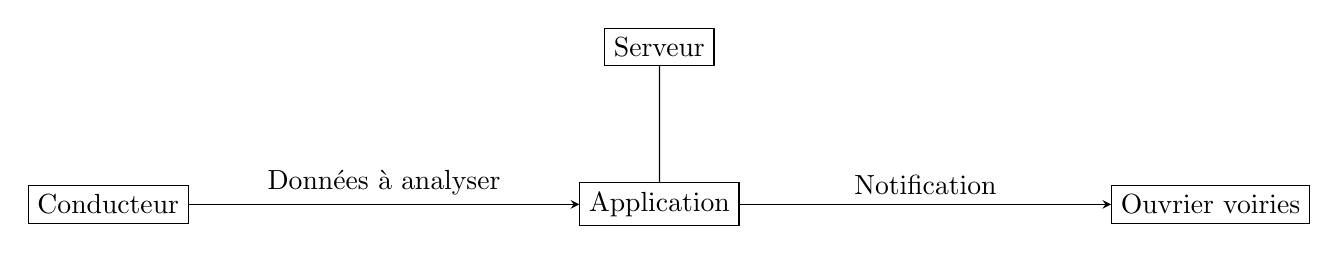
\begin{tikzpicture}[>=stealth,yscale=2,xscale=1.4]
        % Nodes
        \node(conducteur) at (0,0)[rectangle,draw,text centered,align=center]
        {Conducteur};
        \node(app) at (5,0)[rectangle,draw,text centered,align=center]
        {Application};
        \node(entretien) at (10,0)[rectangle,draw,text centered,align=center]
        {Ouvrier voiries};
        \node(serveur) at (5,1)[rectangle,draw,text centered,align=center]
        {Serveur};
        % Links
        \draw[->] (conducteur) -- (app) node[midway,above]{Données à analyser};
        \draw[->] (app) -- (entretien) node[midway,above]{Notification};
        \draw[-] (app) -- (serveur);
    \end{tikzpicture}
    \caption{Description du fonctionnement du système (Analyse)}
    \label{analyse}
\end{figure}

Le traitement des données sur le serveur repose sur un système d'intelligence artificelle permettant de classer les signaux accélérométriques reçus. Etant donné que le modèle est uniquement sur le serveur, il peut facilement être amélioré avec de nouvelles données d'entrainement. Pour cela, un ouvrier peut confirmer une dégradation signalée par l'application. Cela permet d'obtenir de nouvelles données labellées.\\

\begin{figure}[H]
    \centering
    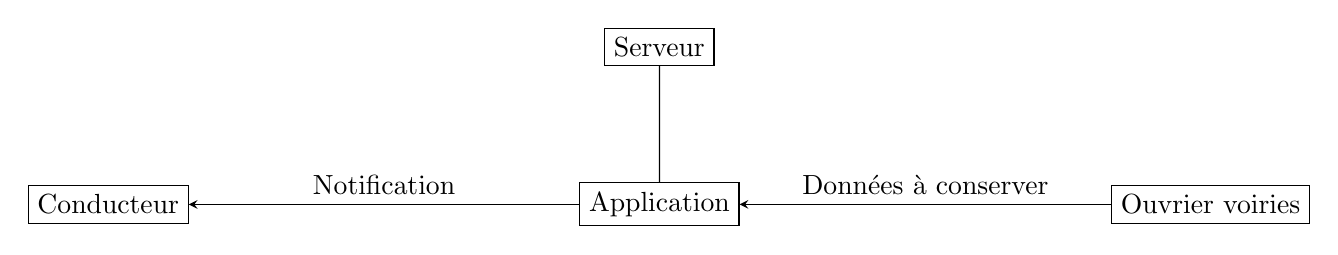
\begin{tikzpicture}[>=stealth,yscale=2,xscale=1.4]
        % Nodes
        \node(conducteur) at (0,0)[rectangle,draw,text centered,align=center]
        {Conducteur};
        \node(app) at (5,0)[rectangle,draw,text centered,align=center]
        {Application};
        \node(entretien) at (10,0)[rectangle,draw,text centered,align=center]
        {Ouvrier voiries};
        \node(serveur) at (5,1)[rectangle,draw,text centered,align=center]
        {Serveur};
        % Links
        \draw[<-] (conducteur) -- (app) node[midway,above]{Notification};
        \draw[<-] (app) -- (entretien) node[midway,above]{Données à conserver};
        \draw[-] (app) -- (serveur);
    \end{tikzpicture}
    \caption{Description du fonctionnement du système (Collecte)}
    \label{collecte}
\end{figure}